\begin{figure}[h]
	\centering
	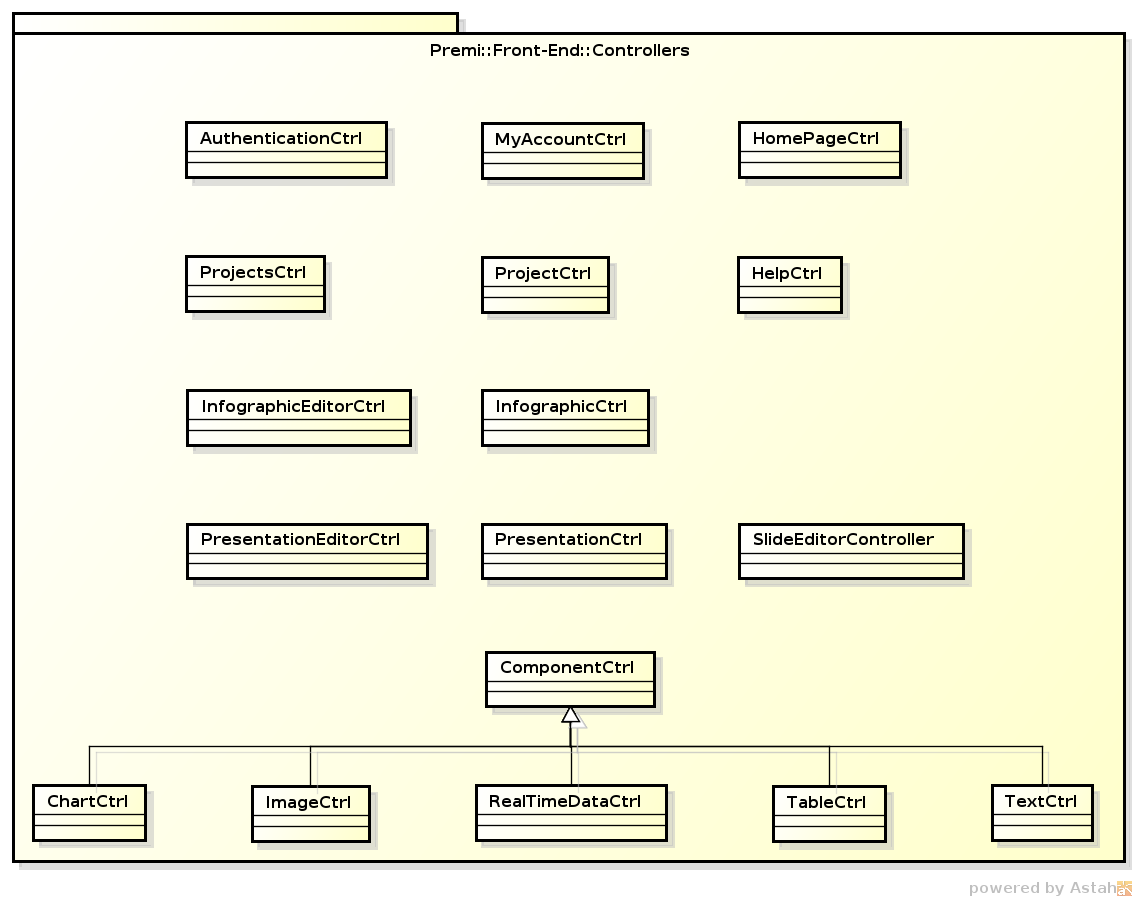
\includegraphics[width=1.0\linewidth]{img/premi_front_end_controllers}
	\caption[Premi::Front-End::Controllers]{Premi::Front-End::Controllers}
\end{figure}
Il package gestisce i controller del front-end dell'applicazione. Comunica con il model, le view e i service della struttura per gestire tutte le operazioni tra di essi. Fa comunicare le view con il model per rendere visibili gli aggiornamenti di quest'ultimo sulle view che utilizzano quei dati. Viceversa, aggiorna il model con le informazioni provenienti dalle view. Richiama inoltre i service per comunicare con il back-end rendendo possibile caricare o salvare i dati nel database.\\
Per brevità la nell'identificare un controller è stata omessa la dicitura Premi::Front-End::Controllers lasciando solamente il nome del controller stesso. Si assume dunque che la dicitura compatta <nomeController> rappresenta la forma estesa Premi::Front-End::Controllers::<nomeController>.

\newpage

\subsubsection{ComponentCtrl}
      \paragraph{Descrizione}
	Il controller ComponentController si occupa di fornire le primitive per la costruzione e gestione dei componenti in una slide.\\
	È una classe astratta in quanto non sarà possibile istanziare un componente direttamente ma solo oggetti che concretizzano la classe costruendo oggetti dei tipi previsti dal sistema.
		
	\paragraph{Utilizzo}
	Questa classe viene utilizzata per consentire all'utente di aggiungere, modificare o rimuovere un componente in una slide.
	
	\paragraph{Attributi}
	\begin{itemize}
		\item \textbf{-\$scope: Object}:\\
			Campo dati contenente un riferimento all'oggetto \$scope creato da Angular, viene utilizzato come mezzo di comunicazione tra il controller e la view. Contiene gli oggetti che definiscono il model dell'applicazione;
		\item\textbf{-x:Double}:\\
			Campo dati contenente il valore della distanza dal bordo sinistro del canvas utilizzata per l'ancoraggio dell'oggetto;
		\item\textbf{-y:Double}:\\
			Campo dati contenente il valore della distanza dal bordo superiore del canvas utilizzata per l'ancoraggio dell'oggetto;
		\item\textbf{-heigth:Double}:\\
			Campo dati contenente il valore dell'altezza dell'oggetto;
		\item\textbf{-width:Double}:\\
			Campo dati contenente il valore della larghezza dell'oggetto;
		\item\textbf{-extraFields:JSON}:\\
			Campo dati contenente eventuali parametri supplementari per ogni componente in un array di oggetti in formato JSON. Progettato in ottica di estensioni future; 
		\item\textbf{-angle:Double}:\\	
			Campo dati contenente il valore dell'angolo di rotazione;
		\item\textbf{-scaleX:Double}:\\
			Campo dati contenente il coefficiente di scala in orizzontale rispetto al valore originale rappresentato dal valore 1;
		\item\textbf{-scaleY:Double}:\\	
			Campo dati contenente il coefficiente di scala in verticale rispetto al valore originale rappresentato dal valore 1.
	
	\end{itemize}
	
	\paragraph{Metodi}
	\begin{itemize}
	\item \textbf{+getX():Double}:\\
		Metodo che restituisce la distanza dal bordo sinistro del canvas utilizzata per l'ancoraggio dell'oggetto selezionato;
	\item \textbf{+getY():Double}:\\
		Metodo che restituisce la distanza dal bordo superiore del canvas utilizzata per l'ancoraggio dell'oggetto selezionato;
	\item \textbf{+getHeigth():Double}:\\
		Metodo che restituisce l'altezza dell'oggetto selezionato;
	\item \textbf{+getWidth():Double}:\\
		Metodo che restituisce la larghezza dell'oggetto selezionato;
	\item \textbf{+getExtraFields():JSON}:\\
		Metodo che restituisce un oggetto JSON con le informazioni aggiuntive dell'oggetto selezionato;
	\item \textbf{+getAngle():Double}:\\
		Metodo che restituisce l'angolo di rotazione dell'oggetto selezionato;
	\item \textbf{+getScaleX():Double}:\\
		Metodo che restituisce il livello di zoom applicato alla larghezza dell'oggetto selezionato;
	\item \textbf{+getScaleY():Double}:\\
		Metodo che restituisce il livello di zoom applicato all'altezza dell'oggetto selezionato;
	\item \textbf{+setX(\textit{value}:Double):Boolean}:\\
		Metodo che permette di impostare la distanza dal bordo sinistro del canvas utilizzata per l'ancoraggio dell'oggetto selezionato al valore \textit{value} restituendo \textit{true} in caso di successo e \textit{false} in caso di fallimento;
	\item \textbf{+setY(\textit{value}:Double):Boolean}:\\
		Metodo che permette di impostare la distanza dal bordo superiore del canvas utilizzata per l'ancoraggio dell'oggetto selezionato al valore \textit{value} restituendo \textit{true} in caso di successo e \textit{false} in caso di fallimento;
	\item \textbf{+setHeigth(\textit{value}:Double):Boolean}:\\
		Metodo che permette di impostare l'altezza dell'oggetto selezionato al valore \textit{value} restituendo \textit{true} in caso di successo e \textit{false} in caso di fallimento;
	\item \textbf{+setWidth(\textit{value}:Double):Boolean}:\\
		Metodo che permette di impostare la larghezza dell'oggetto selezionato al valore \textit{value} restituendo \textit{true} in caso di successo e \textit{false} in caso di fallimento;
	\item \textbf{+setExtraFields(\textit{obj}:JSON):Boolean}:\\
		Metodo che permette di impostare le proprietà aggiuntive dell'oggetto selezionato prendendo i valori dall'oggetto JSON \textit{obj} passato per parametro restituendo \textit{true} in caso di successo e \textit{false} in caso di fallimento;
	\item \textbf{+setAngle(\textit{value}:Double):Boolean}:\\
		Metodo che permette di impostare l'angolo di rotazione dell'oggetto selezionato al valore \textit{value} restituendo \textit{true} in caso di successo e \textit{false} in caso di fallimento;
	\item \textbf{+setScaleX(\textit{value}:Double):Boolean}:\\
		Metodo che permette di impostare il livello di zoom applicato alla larghezza dell'oggetto selezionato al valore \textit{value} restituendo \textit{true} in caso di successo e \textit{false} in caso di fallimento;
	\item \textbf{+setScaleY(\textit{value}:Double):Boolean}:\\
		Metodo che permette di impostare il livello di zoom applicato all'altezza dell'oggetto selezionato al valore \textit{value} restituendo \textit{true} in caso di successo e \textit{false} in caso di fallimento.
	\end{itemize}
	\paragraph{Relazioni con altre classi}
	\begin{itemize}
	 \item OUT: \textbf{SlideEditorCtrl}:\\
		Il controller SlideEditorCtrl utilizza ComponentController per la gestione dei componenti al fine di costruire la slide.
	 \item OUT: \textbf{ChartCtrl}:\\
	 	Il controller ChartCtrl estende ComponentController per la costruzione e gestione di grafici.
	 \item OUT: \textbf{ImageCtrl}:\\
		Il controller ImageCtrlController estende ComponentController per la costruzione e gestione di oggetti di tipo immagine.
	 \item OUT: \textbf{RealTimeDataCtrl}:\\
		Il controller RealTimeDataCtrl estende ComponentController per la costruzione e gestione di oggetti con aggiornamento in tempo reale.
	 \item OUT: \textbf{TableCtrl}:\\
		Il controller TableCtrl estende ComponentController per la costruzione e gestione di oggetti di tipo tabella.
	 \item OUT: \textbf{TextCtrl}:\\
		Il controller TextCtrl estende ComponentController per la costruzione e gestione di oggetti di tipo testo.
	
	\end{itemize}
\newpage
\subsubsection{HelpCtrl}
      \paragraph{Descrizione}
	Il controller HelpCtrl gestisce i meccanismi di aiuto all'utente.
	
	\paragraph{Utilizzo}
	Questa classe viene utilizzata per gestire le informazioni e la logica di erogazione degli aiuti all'utente sotto forma di suggerimenti(tips) esplicativi delle funzionalità.
	
	\paragraph{Attributi}
	\begin{itemize}
		\item \textbf{-\$scope: Object}:\\
				Campo dati contenente un riferimento all'oggetto \$scope creato da Angular, viene utilizzato come mezzo di comunicazione tra il controller e la view. Contiene gli oggetti che definiscono il model dell'applicazione.
		\item \textbf{-\$scope.tips: JSON}:\\
				Campo dati che racchiude in un array di oggetti JSON tutti i suggerimenti necessari allo svolgimento del tour tra le funzionalità del sistema ed al supporto all'utente. 
	\end{itemize}
	
	\paragraph{Metodi}
	\begin{itemize}
	  \item \textbf{+setTips(\textit{obj}:JSON):Boolean}:\\
		  Metodo che permette di aggiungere uno o più suggerimenti tramite un oggetto JSON. Il metodo restituisce \textit{true} in caso di successo e \textit{false} in caso di fallimento;
	  \item \textbf{+getTips():JSON}:\\
		  Metodo che restituisce tutti i suggerimenti in un oggetto JSON.
	\end{itemize}
	\paragraph{Relazioni con altre classi}
	\begin{itemize}
	 \item OUT: \textbf{Views::SlideEditor}:\\
		La vista SlideEditorCtrl utilizza HelpCtrl per la gestione degli aiuti nella composizione e modifica di una slide.
	 \item OUT: \textbf{Views::InfographicEditor}:\\
		La vista Views::InfographicEditor utilizza HelpCtrl per la gestione degli aiuti nella composizione e modifica di una infografica.
	 \item OUT: \textbf{Views::Projects}:\\
		La vista Views::Projects utilizza HelpCtrl per la gestione degli aiuti nella gestione dei progetti dell'utente.
	 \item OUT: \textbf{Views::Search}:\\
		La vista SearchView utilizza HelpCtrl per la gestione degli aiuti nella ricerca di progetti.
	\end{itemize}

\newpage
\subsubsection{InfographicEditorCtrl}
	\paragraph{Descrizione}
		Il controller InfographicEditorCtrl gestisce la composizione e modifica di una infografica sulla base di template predefiniti che permettono l'inserimento in posizioni specifiche di slide precedentemente create.
	
	\paragraph{Utilizzo} 
	
		Questa classe viene utilizzata per gestire le richieste da parte della vista InfographicEditor ed aggiornarla a seconda delle modifiche della classe Premi::Front-End::Model::Infographic.
		Ha il compito di tener traccia ed aggiornare codice identificativo e posizione delle slide in un template di infografica.
	\paragraph{Attributi}
	\begin{itemize}
		\item \textbf{-\$scope: Object}:\\
			Campo dati contenente un riferimento all'oggetto \$scope creato da Angular, viene utilizzato come mezzo di comunicazione tra il controller e la view. Contiene gli oggetti che definiscono il model dell'applicazione.
		\item \textbf{-InfographicService: InfographicService}:\\
			Campo dati che contiene un riferimento al servizio che si occupa di reperire e salvare le informazioni di una infografica.
	\end{itemize}
	
	\paragraph{Metodi}
	\begin{itemize}
	  \item \textbf{+addElement(\textit{position}:Int, \textit{id}:Int):Boolean}:\\
		  Metodo che permette di aggiungere l'elemento con codice identificativo \textit{id} alla infografica in posizione \textit{position}.
	  \item \textbf{+getElement(\textit{position}:Int):Int}:\\
		  Metodo che restituisce il codice identificativo dell'oggetto in posizione \textit{position} in caso di successo e \textit{-1} in caso di fallimento.
	  \item \textbf{+removeElement(\textit{position}:Int):Boolean}:\\
		  Metodo che elimina l'oggetto in posizione \textit{position} restituendo \textit{true} in caso di successo e \textit{false} in caso di fallimento.
	  \item \textbf{+setTemplate(\textit{Tid}:Int):Boolean}:\\
		  Metodo che imposta il template \textit{Tid} per l'infografica corrente nella vista InfographicEditor restituendo \textit{true} in caso di successo e \textit{false} in caso di fallimento.
	  \item \textbf{+getSlideList():JSON}:\\
		  Metodo che restituisce un oggetto JSON contenente un array con tutte le slide dell'infografica con le relative posizioni nel template.
		  
	\end{itemize}
	\paragraph{Relazioni con altre classi}
	\begin{itemize}
		\item IN: \textbf{InfographicService};
		\item IN: \textbf{HelpCtrl};
		\item OUT: \textbf{Views::InfographicEditor}:\\
			La vista InfographicEditor utilizza HelpCtrl per la gestione degli aiuti nella composizione e modifica di una infografica. 	
	\end{itemize}
	
\subsubsection{AuthenticationCtrl}	
\paragraph{Descrizione}
	Il controller AuthenticationCtrl gestisce l'autenticazione di un utente nel sistema.
	
	\paragraph{Utilizzo}
	Questa classe viene utilizzata per gestire le richieste di autenticazione, disconnessione e gestione password all'interno del sistema e di regolare l'accesso alle aree riservate.
	In particolare gestisce le operazioni di logIn, logOut e recupero Password.
	\paragraph{Attributi}
	\begin{itemize}
		\item \textbf{-\$scope: Object}:\\
			Campo dati contenente un riferimento all'oggetto \$scope creato da Angular, viene utilizzato come mezzo di comunicazione tra il controller e la view. Contiene gli oggetti che definiscono il model dell'applicazione.
		\item \textbf{-AuthenticationService: AuthenticationService}:\\
			Campo dati che contiene un riferimento al servizio che si occupa di gestire le funzionalità di autenticazione nel sistema.
	\end{itemize}
	
	\paragraph{Metodi}
	\begin{itemize}
	  	\item \textbf{+logIn(\textit{username}:String, \textit{Password}:String):Boolean}:\\
		 	Metodo che permette di autenticare l'utente con username \textit{username} nel sistema verificando le sue credenziali;
	  	\item \textbf{+logOut(\textit{username}:String):Boolean}:\\
		  	Metodo che permette di disconnettere l'utente con username \textit{username} dal sistema restituendo \textit{true} in caso di successo e \textit{false} in caso di fallimento;
	  	\item \textbf{+forgotPassword(\textit{username}:String):void}:\\
		  	Metodo che si occupa di fornire il supporto al recupero password dell'utente con username \textit{username}.
	   	\item \textbf{+register(\textit{username}:String,\textit{password}:String):Boolean}:\\
	  		Metodo che esegue la procedura di registrazione di un nuovo utente con username \textit{username} e password \textit{password} restituendo \textit{true} in caso di successo e \textit{false} in caso di fallimento;
	  	\item \textbf{+registerViaFacebook()(\textit{name}:Boolean}:\\
	  		 Metodo che esegue la procedura di registrazione di un nuovo utente con le API di Facebook restituendo \textit{true} in caso di successo e \textit{false} in caso di fallimento;
	  	\item \textbf{+registerViaGooglePlus()(\textit{query}:Boolean}:\\
	  		 Metodo che esegue la procedura di registrazione di un nuovo utente con le API di Google+ restituendo \textit{true} in caso di successo e \textit{false} in caso di fallimento;
	\end{itemize}
	\paragraph{Relazioni con altre classi}
	\begin{itemize}
	  \item OUT: \textbf{Views::InfographicEditor}:\\
		La vista Views::InfographicEditor utilizza AuthenticationCtrl per autorizzare un utente alla composizione e modifica di una infografica;	
	  \item OUT: \textbf{Views::PresentationEditor}:\\
		La vista Views::PresentationEditor utilizza AuthenticationCtrl per autorizzare un utente alla composizione e modifica di una presentazione;
	  \item OUT: \textbf{Views::SignUp}:\\
		La vista Views::SignUp utilizza AuthenticationCtrl per gestire permettere al sistema di registrare un nuovo utente;
	  \item OUT: \textbf{Views::LogIn}:\\
	  		La vista Views::LogIn utilizza AuthenticationCtrl per gestire permettere ad un utente di accreditarsi nel sistema;
	  \item IN: \textbf{AuthenticationService}.	
	  \item OUT: \textbf{Views::Project}:\\
		La vista Views::Project utilizza AuthenticationCtrl per autorizzare un utente alla creazione e modifica di un progetto;	
	  \item IN: \textbf{Model::User}:\\
		Classe del model che gestisce gli utenti e le loro informazioni comprensive di quelle di autenticazione;
	  \item IN: \textbf{AuthenticationService}.
	  
	\end{itemize}	
	
\newpage
\subsubsection{PresentationCtrl}
	\paragraph{Descrizione}
	Il controller PresentationCtrl gestisce la creazione e modifica e visualizzazione di una presentazione.
	
	\paragraph{Utilizzo}
	Questa classe viene utilizzata per gestire le richieste da parte della vista Views::Presentation ed aggiornarla a seconda delle modifiche della classe Premi::Front-End::Model::Presentation. PresentationCtrl ha la responsabilità di rendere persistenti le modifiche di un progetto nel front-end anche nel back-end mediante una chiamata al servizio PresentationService.
	Ha il compito di tener traccia delle slide da visualizzare e delle rispettive posizioni\footnote{La presentazione è organizzata secondo una griglia, quindi per ogni slide è necessario salvare le coordinate X e Y.}.
	\paragraph{Attributi}
	\begin{itemize}
		\item \textbf{-\$scope: Object}:\\
			Campo dati contenente un riferimento all'oggetto \$scope creato da Angular, viene utilizzato come mezzo di comunicazione tra il controller e la view. Contiene gli oggetti che definiscono il model dell'applicazione.
		\item \textbf{-PresentationService: PresentationService}:\\
			Campo dati che contiene un riferimento al servizio che si occupa di reperire le informazioni necessarie alla vista Views::Presentation e di fornire le funzionalità necessarie alla corretta erogazione della presentazione.
		\item \textbf{-\$scope.slides: JSON}:\\
			Campo dati che contiene sottoforma di array di oggetti JSON tutte le slide appartenenti alla presentazione. Ogni slide è corredata dalle coordinate cartesiane di posizionamento sulla griglia.
		
		\item \textbf{-\$scope.theme: String}:\\
			Campo dati che contiene un riferimento alla configurazione grafica che l'utente ha scelto come predefinita per la sua presentazione.
		
		\item \textbf{-\$scope.transition: String}:\\
			Campo dati che contiene un riferimento alla tipologia di transizione tra slide che l'utente ha scelto come predefinita per la sua presentazione.
	\end{itemize}
	
	\paragraph{Metodi}
	\begin{itemize}
	  \item \textbf{+setPresentation(\textit{id}:Int):Boolean}:\\
		  Metodo che imposta la presentazione identificata da  \textit{id} per la corretta erogazione da parte della vista Views::Presentation restituendo \textit{true} in caso di successo e \textit{false} in caso di fallimento;
	  \item \textbf{+getPresentation():JSON}:\\
		  Metodo che restituisce un array di oggetti JSON contenente un array con tutte le slides della presentazione con le relative coordinate nella presentazione.
		  
	\end{itemize}
	\paragraph{Relazioni con altre classi}
	\begin{itemize}
	  \item OUT: \textbf{Views::Presentation}:\\
		La vista Views::InfographicEditor utilizza HelpCtrl per la gestione degli aiuti nella composizione e modifica di una infografica;	
	  \item IN: \textbf{PresentationService}: \\
	  	Il servizio PresentationService viene utilizzato per il reperimento ed il salvataggio di una presentazione.
	\end{itemize}
	
\newpage	
\subsubsection{PresentationEditorCtrl}
\begin{figure}[h]
	\centering
	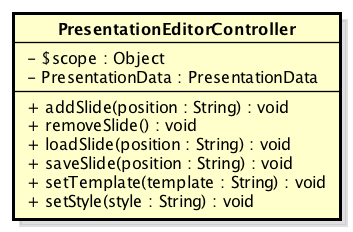
\includegraphics[width=0.5\linewidth]{img/premi_front_end_controllers_presentationeditorcontroller}
	\caption[Premi::Front-End::Controllers::PresentationEditorCtrl]{Premi::Front-End::Controllers::PresentationEditorCtrl}
\end{figure}

	\paragraph{Descrizione}
	Il controller PresentationEditorCtrl si occupa della modifica di una presentazione con i metodi per gestire le slide.
	
	\paragraph{Utilizzo}
	Questa classe viene utilizzata per consentire all'utente di aggiungere o rimuovere una slide dalla presentazione in una posizione qualsiasi e spostarsi tra di esse. Permette inoltre di impostare lo stile e il template della presentazione.
	
	\paragraph{Attributi}
	\begin{itemize}
		\item \textbf{- PresentationService: PresentationService}:\\
			Campo dati che contiene un riferimento al servizio che si occupa della gestione dei dati e delle impostazioni di una presentazione;
		\item \textbf{- \$scope: Object}:\\
			Campo dati contenente un riferimento all'oggetto \$scope creato da Angular, viene utilizzato come mezzo di comunicazione tra il controller e la view. Contiene gli oggetti che definiscono il model dell'applicazione.
		\item \textbf{- \$scope.currentPresentation: JSON}:\\
			Campo dati che contiene un array di oggetti JSON contenenti le informazioni della presentazione corrente;		
		
	\end{itemize}
	
	\paragraph{Metodi}
	\begin{itemize}
		\item \textbf{addSlide(direction: String):Boolean}:\\
			Metodo che aggiunge una slide alla presentazione rispetto alla slide corrente nella posizione indicata da \textit{direction}\footnote{Per \textit{direction} si intende la direzione nella quale si vuole aggiungere o caricare una slide\{up, right, down, left\}}. Il metodo restituisce \textit{true} in caso di successo e \textit{false} in caso di fallimento;
		\item \textbf{removeSlide():Boolean}:\\
			Metodo che rimuove la slide corrente dal canvas di modifica restituendo \textit{true} in caso di successo e \textit{false} in caso di fallimento;
		\item \textbf{loadSlide(direction: String):Boolean}\\
			Metodo che carica la slide nella posizione indicata da \textit{direction} nel canvas di modifica restituendo \textit{true} in caso di successo e \textit{false} in caso di fallimento;
		\item \textbf{saveSlide():Boolean}\\
			Metodo che salva la slide correntemente caricata sul canvas di modifica restituendo \textit{true} in caso di successo e \textit{false} in caso di fallimento;
		\item \textbf{setTheme(theme: String):Boolean}
			Metodo che imposta l'aspetto grafico predefinito per la presentazione al valore passato per parametro restituendo \textit{true} in caso di successo e \textit{false} in caso di fallimento;
		\item \textbf{setTransition(transition: String):Boolean}
			Metodo che imposta lo stile di transizione tra slide al valore passato per parametro restituendo \textit{true} in caso di successo e \textit{false} in caso di fallimento.
	\end{itemize}
	\paragraph{Relazioni con altre classi}
	\begin{itemize}
	  \item OUT: \textbf{Views::PresentationEditor}:\\
		La vista Views::PresentationEditor utilizza PresentationEditorCtrl per la gestione delle slide nella composizione e modifica di una presentazione;	
	  \item IN: \textbf{PresentationService}.
	  \item IN: \textbf{Views::SlideEditor}.
	  \item IN: \textbf{SlideEditorCtrl}.
	\end{itemize}  
\newpage
\subsubsection{ProjectCtrl}
	\paragraph{Descrizione}
	Il controller ProjectCtrl gestisce il progetto corrente.
	
	\paragraph{Utilizzo}
	Questa classe viene utilizzata per modificare un progetto esistente\footnote{Un progetto vuoto viene creato di default con una presentazione vuota.}.\\
	Permette di aggiungere infografiche, richiamare le funzionalità di modifica di infografiche e della presentazione. Inoltre permette di lanciare la vista di visualizzazione della presentazione.
	\paragraph{Attributi}
	\begin{itemize}
		\item \textbf{-\$scope: Object}:\\
			Campo dati contenente un riferimento all'oggetto \$scope creato da Angular, viene utilizzato come mezzo di comunicazione tra il controller e la view. Contiene gli oggetti che definiscono il model dell'applicazione;
		\item \textbf{-\$scope.presentation: JSON}:\\
			Campo dati contenente un riferimento alla presentazione appartenente al progetto corrente;
		\item \textbf{-\$scope.infographics: JSON}:\\
			Campo dati contenente un array di oggetti JSON ognuno rappresentante una infografica del progetto corrente;	
		\item \textbf{-ProjectService: ProjectService}:\\
			Campo dati che contiene un riferimento al servizio che si occupa di reperire le informazioni necessarie al corretto funzionamento della vista Views::Project.
	\end{itemize}
	
	\paragraph{Metodi}
	\begin{itemize}
	  	\item \textbf{+setPresentation(\textit{id}:Int):Boolean}:\\
		  	Metodo che imposta la presentazione identificata da  \textit{id} per la corretta erogazione della presentazione da parte della vista Views::Presentation restituendo \textit{true} in caso di successo e \textit{false} in caso di fallimento;
	  	\item \textbf{+getPresentation():JSON}:\\
		  	Metodo che restituisce un oggetto JSON contenente un array con tutte le slide della presentazione con le relative coordinate nella presentazione;
	 	\item \textbf{+resetPresentation():Boolean}:\\
			Metodo che riporta la presentazione relativa al progetto corrente allo stato iniziale ovvero dotata di una sola slide vuota restituendo \textit{true} in caso di successo e \textit{false} in caso di fallimento;
		\item \textbf{+addInfographic():Int}:\\
			Metodo che inserisce ua nuova infografica al progetto corrente restituendone il codice identificativo;
		\item \textbf{+deleteInfographic(\textit{id}:Int):Boolean}:\\
	  		Metodo che elimina l'infografica identificata da \textit{id} dal progetto corrente restituendo \textit{true} in caso di successo e \textit{false} in caso di fallimento.
		
		  
	\end{itemize}
	\paragraph{Relazioni con altre classi}
	\begin{itemize}
	  \item OUT: \textbf{Views::Project}:\\
		La vista Views::Project utilizza ProjectCtrl per la gestione reperire ed aggiornare le informazioni di pertinenza del progetto corrente;	
	  \item IN: \textbf{ProjectService}.
		La vista Views::Project utilizza il service ProjectService per reperire ed aggiornare le informazioni di pertinenza del progetto corrente dal back-end.
	\end{itemize}

\newpage
\subsubsection{ProjectsCtrl}
	\paragraph{Descrizione}
	Il controller ProjectsCtrl gestisce i progetti dell' utente corrente.
	
	\paragraph{Utilizzo}
	Questa classe viene utilizzata per visualizzare tutti i progetti dell'utente corrente, lanciarne la modalità di modifica (gestita da ProjectCtrl) e crearne di nuovi.\\
	\paragraph{Attributi}
	\begin{itemize}
		\item \textbf{-\$scope: Object}:\\
			Campo dati contenente un riferimento all'oggetto \$scope creato da Angular, viene utilizzato come mezzo di comunicazione tra il controller e la view. Contiene gli oggetti che definiscono il model dell'applicazione;
		\item \textbf{-ProjectService: ProjectService}
	\end{itemize}
	
	\paragraph{Metodi}
	\begin{itemize}
	  \item \textbf{+setPresentation(\textit{id}:Int):void}:\\
		  Metodo che imposta la presentazione identificata da  \textit{id} per la corretta erogazione della presentazione da parte della vista Views::Presentation;
	  \item \textbf{+getProject(\textit{id}:Int):JSON}:\\
		  Metodo che restituisce un oggetto JSON contenente un array con la presentazione e tutte le infografiche del progetto identificato da \textit{id}.
		  
	\end{itemize}
	\paragraph{Relazioni con altre classi}
	\begin{itemize}
	  \item OUT: \textbf{Views::Projects}:\\
		La vista Views::Projects utilizza ProjectsCtrl per la gestione reperire ed aggiornare le informazioni di pertinenza dei progetti dell'utente corrente;	
	  \item IN: \textbf{ProjectService}.
		La vista Views::Projects utilizza il service ProjectService per reperire ed aggiornare le informazioni di pertinenza dei progetti dell'utente corrente dal back-end.
	\end{itemize}	




































%
%\newpage	
%\subsubsection{SearchController}
%	\paragraph{Descrizione}
%	Il controller SearchController gestisce le funzionalità di ricerca del sistema.
%	
%	\paragraph{Utilizzo}
%	Questa classe viene utilizzata per visualizzare tutti i risultati di ricerca a seguito di una interrogazione da parte di utente qualunque.\\
%	\paragraph{Attributi}
%	\begin{itemize}
%		\item \textbf{-\$scope: Object}:\\
%			Campo dati contenente un riferimento all'oggetto \$scope creato da Angular, viene utilizzato come mezzo di comunicazione tra il controller e la view. Contiene gli oggetti che definiscono il model dell'applicazione;
%		\item \textbf{-ProjectService: ProjectService}
%			Campo dati che contiene un riferimento al servizio che si occupa di gestire le funzionalità di gestione di un progetto nel sistema.
%	\end{itemize}
%	
%	\paragraph{Metodi}
%	\begin{itemize}
%	  \item \textbf{+searchUsers(\textit{username}:String):JSON}:\\
%		  Metodo ritorna un oggetto JSON contenente un array di tutti i progetti dell'utente con username \textit{username};
%	  \item \textbf{+searchProject(\textit{name}:String):JSON}:\\
%		  Metodo ritorna un oggetto JSON contenente un array di tutti i progetti il cui nome ha un match con \textit{name};
%	  \item \textbf{+search(\textit{query}:String):JSON}:\\
%		  Metodo ritorna un oggetto JSON contenente un array di tutti i progetti il cui nome ha un match con \textit{name} e dell'utente con username \textit{username};
%		  
%	\end{itemize}
%	\paragraph{Relazioni con altre classi}
%	\begin{itemize}
%	  \item OUT: \textbf{SearchView}:\\
%		La vista SearchView utilizza ProjectsCtrl per la gestione reperire ed aggiornare le informazioni di pertinenza dei progetti che hanno un match con il nome del progetto oppure con lo username dell'utente;	
%	  \item IN: \textbf{ProjectService}.
%		La vista SearchView utilizza il service ProjectService per reperire ed aggiornare le informazioni di pertinenza dei progetti dal back-end che hanno un match con il nome del progetto oppure con lo username dell'utente proprietario a seguito di un'interrogazione.	
%	\end{itemize}		
%	
\newpage
	
\subsubsection{SlideEditorCtrl}
	\paragraph{Descrizione}
	Il controller SlideEditorCtrl gestisce le funzionalità di modifica di una slide.
	
	\paragraph{Utilizzo}
	Questa classe viene utilizzata per permettere alla vista Views::SlideEditor di inserire componenti in un a slide, modificarne le caratteristiche oppure eliminarli.\\
	\paragraph{Attributi}
	\begin{itemize}
		\item \textbf{-\$scope: Object}:\\
			Campo dati contenente un riferimento all'oggetto \$scope creato da Angular, viene utilizzato come mezzo di comunicazione tra il controller e la view. Contiene gli oggetti che definiscono il model dell'applicazione;
		\item \textbf{-SlideService: SlideService}:\\
			Campo dati che contiene un riferimento al servizio che si occupa di gestire le funzionalità di modifica e gestione di una slide.
		\item \textbf{-PresentationService: PresentationService}:\\
			Campo dati che contiene un riferimento al servizio che si occupa di gestire le funzionalità di modifica e gestione di una Presentazione.
	\end{itemize}
	
	\paragraph{Metodi}
	\begin{itemize}
	  \item \textbf{+addObject():Int}:\\
		 Metodo che esegue la procedura di aggiunta di un nuovo componente nella slide corrente mediante una chiamata al service PresentationService ritornando il codice identificativo \textit{id}.
	  \item \textbf{+udpateObject(\textit{id}:String):Boolean}:\\
		 Metodo che esegue la procedura di aggiornamento di un componente  identificato da \textit{id} nella slide corrente mediante una chiamata al service PresentationService  restituendo \textit{true} in caso di successo e \textit{false} in caso di fallimento.\\I valori sono reperiti dalla variabile \$scope.selectedObject;
	  \item \textbf{+removeObject(\textit{id}:String):Boolean}\\
		 Metodo che esegue la rimozione del componente identificato da \textit{id} nella slide corrente mediante una chiamata al service SlideService  restituendo \textit{true} in caso di successo e \textit{false} in caso di fallimento.
	  \item \textbf{+saveSlide(\textit{id}:Int):Boolean}:\\
		 Metodo che esegue la procedura di salvataggio della slide corrente mediante una chiamata al service SlideService restituendo \textit{true} in caso di successo e \textit{false} in caso di fallimento.
	  \item \textbf{+loadSlide(\textit{id}:Int):Boolean}:\\
		 Metodo che esegue la procedura di caricamento della slide corrente mediante una chiamata al service PresentationService restituendo \textit{true} in caso di successo e \textit{false} in caso di fallimento.
	  	  
	\end{itemize}
	\paragraph{Relazioni con altre classi}
	\begin{itemize}
	  \item OUT: \textbf{Views::SlideEditor}:\\
		La vista Views::SlideEditor utilizza SlideEditorCtrl per la gestione reperire ed aggiornare le informazioni di pertinenza della slide corrente;	
	  \item IN: \textbf{SlideService}.
		La vista Views::SlideEditor utilizza il service SlideService per recuperare ed aggiornare le informazioni della slide corrente sul Back-End.	
	  \item IN: \textbf{PresentationService}.
		La vista Views::SlideEditor utilizza il service PresentationService recuperare la posizione della slide nella presentazione ed aggiornare i suoi indici sincronizzandosi con il Back-End.	
	\end{itemize}		
	
	
% 	SlideService
% PresentationService
% addObject(id)
% removeObject(id)